\documentclass[12pt,a4paper]{report}
\usepackage{graphicx}
\usepackage[francais]{babel}
\usepackage[utf8]{inputenc}
\usepackage[T1]{fontenc}
\usepackage{alltt}
\usepackage{fancyhdr}
\setlength{\headheight}{15.2pt}
\pagestyle{fancy}
  
\title{Rapport de soutenance \no{2}} 
\date{}
\author{TeGaSz}
\newcommand{\HRule}{\rule{\linewidth}{0.5mm}}



\begin{document}

\begin{titlepage}



\begin{center}



\textsc{\LARGE PROJET}\\[1.5cm]

\textsc{\Large TeGaSz}\\[0.5cm]


% Title
\HRule \\[0.4cm]
{ \huge \bfseries Rapport de Soutenance 2}\\[0.4cm]
  
\HRule \\[1.5cm]

\includegraphics[width=0.6\textwidth]{./name.jpg}\\[1cm]  
% Author and supervisor
\begin{minipage}{0.4\textwidth}
\begin{flushleft} \large
Julien \textsc{Garagnon}\\
Julien \textsc{Szkudlarek}
\end{flushleft}
\end{minipage}
\begin{minipage}{0.4\textwidth}
\begin{flushright} \large
Maxime \textsc{Templé}\\

\end{flushright}
\end{minipage}

\vfill

% Bottom of the page
{\large 17 avril 2012}

\end{center}

\end{titlepage}
\tableofcontents

\chapter{Introduction}

Ceci est le rapport de soutenance du projet réalisé par l'équipe \emph{TeGaSz}. 
Ce dernier se prénomme \emph{P.R.O.J.E.T} (Programme Radiophonique Orienté Jouant Énormémentsur les Tonalités) et est en définitive un lecteur Audio programmé pour fonctionner sous Fedora. \\
Dans ce rapport, nous allons vous présenter notre projet terminé ainsi
que toute la démarche de sa conception, qu'elle soit intellectuelle, sous forme de 
recherche ou tout simplement en code pur.

\chapter{Le projet}
Un lecteur audio est une sorte de lecteur multimédia utilisé pour la lecture audio numérique, les disques optiques tels que CD, SACD, DVD-Audio, HDCD, ou encore  des fichier ou du streaming.

En plus des fonctions de telles que la lecture,la pause,l' arrêt, rembobinage, et la transmission, certaines fonctions courantes comprennent playlisting, support du format de marquage, ou encore un égaliseur.
La plupart des lecteurs audio prennent également en charge la lecture simple des vidéos numériques. ils peuvent également lire des films.

\begin{center}
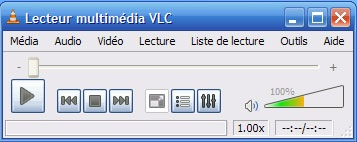
\includegraphics{vlc-interface1.jpg}

\it{un lecteur audio reconnu : VLC}
\end{center}

\section{Les origines du projet}

Le groupe TeGaSz est un groupe de projet formé en 2012 par trois étudiants
d'EPITA passionnés, dans le but de réaliser pour la fin de l'année un
travail de programmation inédit. Ce programme est un lecteur audio codé
dans la majeure partie en C et en Ocaml. Le projet sera accompagné d'un
site web qui décrira tout au long de l'année l'avancement du projet. Il sera
mis à jour régulièrement après chaque évolution notable. Ce projet sera particuli
èrement diffcile à réaliser au niveau de la programmation : En effet, ce
projet demande des notions particulièrement avancées dans le domaine du
cryptage des fichiers audio. Par exemple, il faudra être capable de distinguer
les en-tête de fichier de type .mp3, ou tout simplement être capable de lire
un son, montrer sons avancement dans le temps, et pourquoi pas, afficher
plusieurs informations sur la musique en cours. C'est pourquoi nous allons
commencer ce projet en progressant étape par étape.

\section{Etude du marché}
Nous nous intéressons principalement aux lecteurs audio libres, puisque c'est à cela que nous espérons arriver. voici quelques uns des logiciels disponibles sur le marché:

\subsubsection{The KMPlayer}

Simple et épuré KMPlayer n'en est pas moins puissant. Ce lecteur Coréen a le vent en poupe et il se dit dans les forums qu'il commence à faire de l'ombre à VLC. Lecteur multimédia, KMPlayer est capable de lire pratiquement tous les formats audio et vidéo nativement. Il est doté d'une très belle interface vraiment simple à  utiliser. A découvrir... Il est gratuit et un patch français est disponible.

\subsubsection{Amarok}

Amarok est un lecteur audio. Il était au départ conçu uniquement pour Linux, mais la migration vers les plateformes Windows et Mac OS X est en cours. C'est\`a ce jour l'un des meilleurs lecteurs audio. 
 Amarok peut lire quasiment n'importe quel type de fichiers audio (MP3, OGG, WMA, FLAC...), permet la création de playlists ce qui le transforme en Jukebox, gère l'édition des tags, grave les CD audio (à condition d'avoir K3B), récupère les pochettes de disques ou les paroles d'un morceau, permet d'uploader votre musique vers de nombreux baladeurs (iPod, Creative NOMAD ou ZEN, Rio Karma...), affiche les informations de Wikipedia sur le groupe que vous écoutez... Bref, Amarok est un outil très puissant.
Il faut disposer d'un moteur de décodage tel que GStreamer ou Xine pour faire fonctionner Amarok : Amarok est en quelque sorte une interface utilisateur. 

\subsubsection{Splayer}

Lecteur multimédia extrêmement léger, Splayer est compact, gratuit, facile à utiliser et capable de lire pratiquement tous les formats audio et vidéo sans avoir besoin de plugins supplémentaires. Il est doté d'une superbe interface que l'on apprécie d'autant plus quand on utilise Splayer pour lire des vidéos. 

\subsubsection{Windows Media Player}

Le format WMA est la réponse de Microsoft au MP3. Face au succès du MP3 et l'engouement des internautes pour ce format, Microsoft a réagi en mettant au point le Windows Media Audio codec en 1999. Les techniques de compression sont semblables à celles utilisées par le standard MP3. Windows Media Player est fourni directement avec Windows depuis Windows 98. Pour obtenir la dernière version, voyez les liens ci-dessous. Windows Media Player permet la lecture des CD audio, des fichiers MP3 et WMA et la visualisation de fichiers vidéo. Il est doté d'un égaliseur 10 bandes, d'un gestionnaire de Playlists qui le transforme en Jukebox. Il permet la compression des fichiers Wave en WMA. On peut aussi procéder à l'extraction des pistes audio d'un CD. Les fichiers obtenus sont directement encodés en WMA (on ne récupère pas les wave). Il existe des skins et des plug-ins pour le transfert vers des baladeurs.

\subsubsection{Winamp}

Premier lecteur MP3 logiciel apparu sur le Web en 1997 et toujours très populaire. Aujourd'hui, Winamp est bien plus qu'un simple lecteur MP3. Il permet la lecture des CD audio, des fichiers MP3, OGG, AAC et WMA sans ajout de plug-ins et ceci pour ne parler que des formats les plus courants. Il peut désormais ripper les pistes d'un CD audio pour les copier sur votre disque dur et graver des CD. Ces deux dernières fonctionnalités sont limitées dans la version gratuite : on peut ripper en x6 et graver en x2 seulement mais c'est possible. Cette limitation ne nous semble pas un gros handicap dans la mesure o\`u il vaut mieux ripper \`a  vitesse lente pour obtenir une bonne qualité d'extraction. Mais revenons \`a  Winamp... Il est doté d'un égaliseur 10 bandes, d'un gestionnaire de Playlists qui le transforme en Jukebox et d'un mini navigateur Web. 
L'ajout de plug-ins étend encore les possibilités de Winamp puisqu'on peut encoder en MP3 ou autre format, visualiser des vidéos au format DivX, lire des fichiers audio de type VQF, Monkey... A tester !

\section{Présentation de l'équipe}
TeGaSz est un projet réalisé par trois étudiants en deuxième année à EPITA.
	\subsection{Maxime Templé}
Il y a maintenant quatre ou cinq ans, j'ai découvert les possibilités que pouvaient donner l'informatique. Malgré quelques notions de C et depuis six mois de Ocaml,et un projet en C\# je n'ai jamais eu l'occasion de m'investir pleinement dans le domaine du son lié à la programmation, mais je compte me servir de ce projet afin d'approfondir mes connaissances dans le domaine.

	\subsection{Julien Garagnon}
Troisième année a l'Epita, troisième spé, et enfin je commence le C. Après l'échec du projet cartographie, j'espère bien me rattraper avec cette fois ci un groupe soudé et motivé. n'ayant pratiquement aucune expérience concernant le son, que ça soit sa lecteur, sa production ou encore sa manipulation, ce projet promet de m'apporter de nombreuses connaissances sur le sujet, connaissances dont je suis toujours avide.

	\subsection{Julien Szkudlarek}
Après un premier projet consistant à réaliser une cartographie 3D avec un grand intérêt principalement lié à la visualisation, celui-ci sera donc un lecteur audio. Il s'annonce tout aussi passionnant car le principe même du projet est un outil très commun et de notre quotidien aujourd'hui. Il va également me permettre de pouvoir approfondir le C que je connais relativement peu. Pouvoir créer son propre lecteur audio est un objectif très stimulant d'autant plus que le sujet est plus libre que le précédent ce qui va permettre une meilleure créativité.

\section{Librairies utilisées}
	\subsection{Fmod}

\begin{center}

\includegraphics[scale =0.5]{fmodex.png}
\end{center}
FMOD est une bibliothèque multiplateforme de gestion du son, pouvant être utilisée au travers de noombreux langages de programmation. Avec le lancement de la version 4.03 la bibliothèque a été renommée FMOD Ex.

	\subsection{GTK}

\begin{center}

\includegraphics[scale =0.5]{GTK.jpg}
\end{center}

GTK+ (The GIMP Toolkit) est un ensemble de bibliothèques logicielles, c'est-à-dire un ensemble de fonctions informatiques, permettant de réaliser des interfaces graphiques. Cette bibliothèque a été développée originellement pour les besoins du logiciel de traitement d'images GIMP. GTK+ est maintenant utilisé dans de nombreux projets, dont les environnements de bureau GNOME, Xfce et ROX.
GTK+ est un projet libre (licence GNU LGPL 2.1) et multiplate-forme.

Même si, au départ GTK+ est écrit en langage C et utilise pourtant le paradigme de la programmation orientée objet. Il est également possible d'utiliser GTK+ dans de nombreux autres langages de programmation: C++ (avec gtkmm), Ada (avec GtkAda), Fortran (avec gtk-fortran), Pascal, PHP, Perl, Ruby, Objective Ocaml, Java, Python, Vala, Seed (JavaScript) ou encore C\# avec la plateforme mono au travers du binding Gtk\#, etc.

\chapter{Le planning}
Pour pouvoir réaliser ce projet dans les temps, nous avons choisi de travailler en groupe au moins une fois par semaine, sur des plages d'horaires communes comme le Vendredi soir ou le jeudi matin. Le reste du travail sera réalisé individuellement par chaque membre de l'équipe en suivant un planning et une répartition organisée des tâches décrite plus bas. Le but de ces réunions hebdomadaires est tout simplement de mettre en commun nos idées et de faire le point sur l'avancée du travail de chacun. Ainsi, chaque semaine un planning pour la semaine suivante sera établi pour chaque membre de l'équipe.

\section{Organisation du travail}

Pour pouvoir réaliser ce projet dans les temps, nous avons choisi de travailler en groupe au moins une fois par semaine, sur des plages d'horaires communes comme le Vendredi soir ou le jeudi matin. Le reste du travail sera réalisé individuellement par chaque membre de l'équipe en suivant un planning et une répartition organisée des tâches décrite plus bas. Le but de ces réunions hebdomadaires est tout simplement de mettre en commun nos idées et de faire le point sur l'avancée du travail de chacun. Ainsi, chaque semaine un planning pour la semaine suivante sera établi pour chaque membre de l'équipe.

\section{répartition des tâches}

Tout au long du semestre, nous nous sommes donnés des tâches précises à faire avancer chacun de notre coté. cependant, le temps avancant et la dead line approchant, chaque personne a quitté son travail pour aller aider un autre membre de l'équipe. Nous pouvons donc dire que tout le monde aura travaillé sur tout le projet.
Dans le projet initial, Julien G devait s'occuper de mettre en place la librairie Fmod, Julien S de l'interfaçage entre le C et le Ocaml et enfin Maxime devait mettre en place 

 graphique.

\section{Le chef de projet}

La personne qui s'occupera tout au long de l'année de la mise en place du projet et de l'organisation des travaux sera Maxime, choisi à l'unanimité. Il sera notre chef de projet, c'est-à-dire le principal intermédiaire entre le jury et le groupe de projet lors des soutenances.

\section{utilisation de git}

\begin{center}

\includegraphics[scale =0.5]{git.png}
\end{center}

il nous fallait un outil fiable afin de partager notre avancé commune. Le gestionnaire de version décentralisé GIT semblait tout destine pour cette tache. Pour cela, nous avons donc créé un dépôt sur le site GitHub qui permet gratuitement d'héberger l'ensemble de nos sources.\\
Git est un logiciel de gestion de versions décentralisé. C'est un logiciel libre créé par Linus Torvalds, le créateur du noyau Linux, et distribué selon les termes de la licence publique générale GNU version 2.


\chapter{Le developpement du projet}
Notre projet s'est développé progressivement. Chaque soutenance était une étape avec de nouvelles améliorations, implémentations et d'autres choses plus ou moins visibles. 
Ces avancées seront développées avec précision dans les chapitres prévus à cet effet.

\section{la première soutenance}

\begin{center}
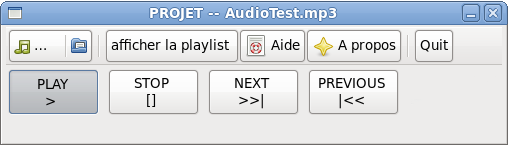
\includegraphics[scale = 0.8]{interface1.png}
\it{ première version du projet}

\end{center}
Lors de cette première soutenance nous nous sommes particulièrement concentré sur l'interfaçage entre le C et le Ocaml parce que cette partie était la plus importante:
Sans elle nous ne pouvions effectuer aucun test! 
Un premier tatonnement sur Fmod aura aussi été fait et l'interface aura été implémentée. 
Au final, nous avions un lecteur audio ne pouvant jouer qu'une seule musique prédéfinie.

\section{la deuxième soutenance}

\begin{center}
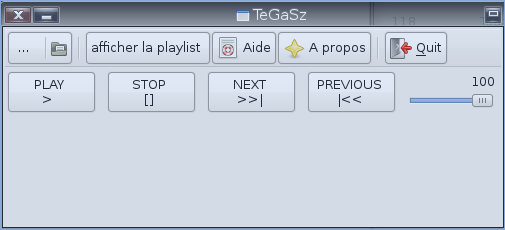
\includegraphics[scale = 0.8]{interface2.png}
\it{ seconde version du projet}
\end{center}


L'interfaçage entre C et Ocaml ayant été implementé pour la première soutenance,  nous pouvions nous concentrer sur le projet en lui-même, à savoir la mise en place de Fmod et son imprecation dans l'interface.
Nous avions donc un lecteur audio plus complexe permettant de charger une chanson, de la lire et de varier le volume.

\section{la soutenance finale}

\begin{center}
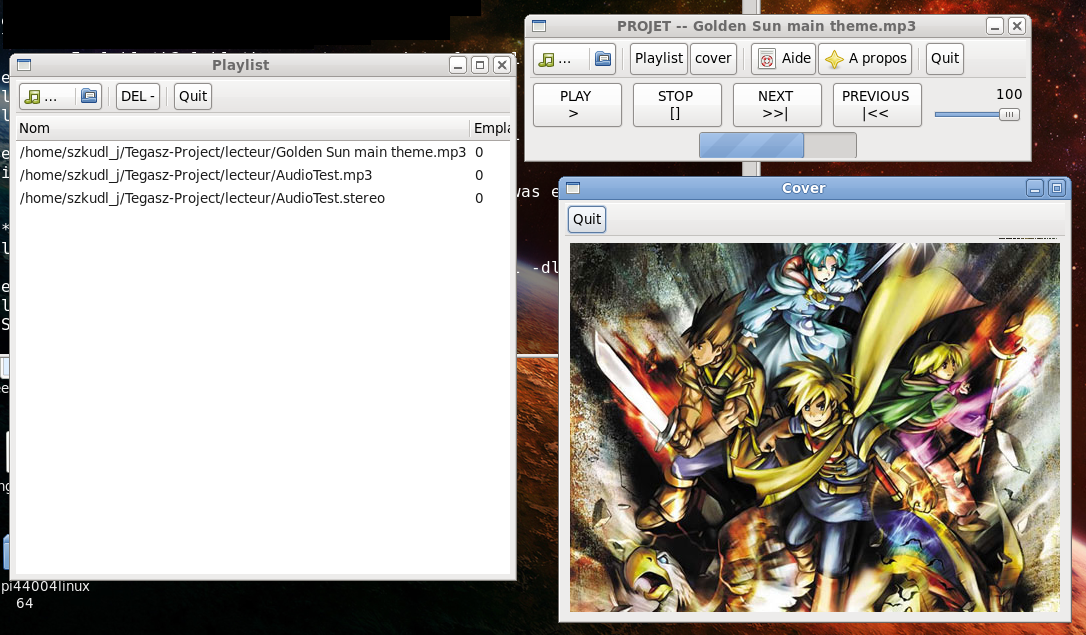
\includegraphics[scale = 0.4]{interface3.png}
\it{visuel final}
\end{center}

\chapter{l'interface}

En informatique, une interface graphique (anglais GUI pour graphical user interface) est un dispositif de dialogue homme-machine, dans lequel les objets à manipuler sont dessinés sous forme de pictogrammes à l'écran, que l'usager peut opérer en imitant la manipulation physique de ces objets avec un dispositif de pointage, le plus souvent une souris.\\

Pour cette dernière version, le principe de base aura été de repartir à
partir des bases posées dans la deuxième soutenance. Nous avons utilisé nos connaissances acquises dans nos recherches pour réaliser une interface qui correspondait beaucoup plus aux attentes du cahier des charges, Bien que les methodes employées pour la plupart des parties restent fondamentalement les memes, nous avons surtout ajouté des actions plus spécifiques, permettant ainsi une meilleure interconnexion entre les différentes parties du projet.

Pour la fin nous avons mis en place les deux nouvelles fenêtres pour la pochette et la playlist.

\section{description des boutons}

L'interface inclue toutes les fonctions que l'on peut attendre d'un lecteur
audio fonctionnel : 
Nous pouvons sélectionner le fichier à charger,lire ce dernier à l'aide du bouton play, un bouton stop pour arrêter la lecture, une barre de volume pour régler l'intensité du son.

 Il y a aussi deux boutons pour changer de piste, bien qui sont fonctionnels pour cette nouvelle soutenance.

Une des particularité du bouton de lecture est qu'il permet aussi de mettre
en pause la lecture.

 Une fois pressé, il reste enfoncé et ainsi l'utilisateur sait que la piste est lue. S'il est de nouveau cliqué, il ressort et la lecture est mise en pause et peut être reprise au même point.

La sélection du volume se fait par une barre coulissante, avec une indication
numérique du volume actuel pour une plus grande précision. A la base,
le volume est indiqué avec une décimale, ainsi pour raison esthétique, nous
avons préféré ne garder que les entiers.

Pour cette nouvelle soutenance, deux nouveaux boutons sont apparus.  le bouton pour afficher la playlist, qui affiche une nouvelle fenêtre contenant bien entendu la liste de lecture, mais aussi un bouton permettant d'ajouter un morceau à la liste, et un autre pour le supprimer.
le second bouton de l'interface permet d'afficher la pochette de l'album.

En ce qui concerne les autres nouveautés, une barre de défilement a été ajoutée.

\section{Architecture de l'interface}



\begin{center}
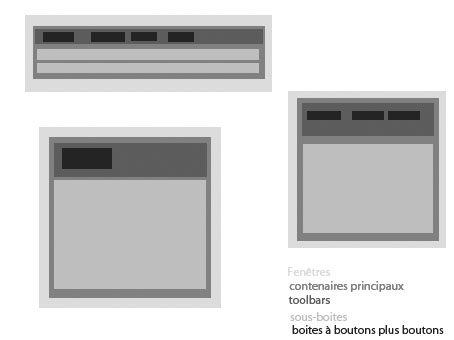
\includegraphics[scale =0.8]{archi.jpg}
\end{center}


Nous pouvons considérer l'interface GTK comme une sorte de Poupée Russe. Il s'agit d'une série de fenêtres et d'imbrications en tout genres.
Tout d'abord nous avons la fenêtre de base, la fenêtre de la playlist et enfin la fenêtre pour la couverture. Contrairement aux deux autres, la première est visible.
Cette dernière contient une boite de boites,contenant elle même une une toolbar, une boite de boutons et une boite de Widgets.La toolbar contient une série d'items contenant chacun un bouton, ou une séparation.
la bouton barre contient les quatres boutons de contrôle et encore une boite de widgets servant à afficher la barre de réglage de volume.

Le troisième élément de  la première boite contient la barre de progression.
une fois cliqué sur le bouton pour afficher la couverture, s'affiche une seconde fenêtre contenant elle aussi un conteneur principal, contenant lui même une toolbar et une boite de fichiers. la toolbar contient une boite de boutons pour afficher le bouton quitter. l'autre boite contient l'image que l'on désire afficher.

Nous procedons de la même façon pour la playlist.


\chapter{Moteur son}
\section{Le Son}


Le son est une onde produite par la vibration mécanique d'un support fluide ou solide et propagée grâce à l'élasticité du milieu environnant sous forme d'ondes longitudinales. Par extension physiologique, le son désigne la sensation auditive à laquelle cette vibration est susceptible de donner naissance.\\
\begin{center}


\includegraphics[scale=0.7]{onde.jpg}

\it{Une onde}
\end{center}

Dans un milieu compressible, le plus souvent dans l'air, le son se propage sous forme d'une variation de pression créée par la source sonore. Un haut-parleur, par exemple, utilise ce mécanisme. Seule la compression se déplace et non les molécules d'air, si ce n'est de quelques micromètres. Lorsque l'on observe des ronds dans l'eau, les vagues se déplacent mais l'eau reste au même endroit, elle ne fait que se déplacer verticalement et non suivre les vagues (un bouchon placé sur l'eau reste à la même position sans se déplacer). Le son se propage également dans les solides sous forme de vibrations des atomes appelées phonons. Là encore, seule la vibration se propage, et non les atomes qui ne font que vibrer très faiblement autour de leur position d'équilibre.\\

Le son en informatique est toujours représenté de manière numérique. De nombreux standards existent; certains s'appliquent à la production, au stockage et à la diffusion, d'autres (ceux qui utilisent des algorithmes de compression de données ou de débit), sont destinés, en principe, uniquement à la diffusion. Actuellement, le format le plus utilisé est de loin le mp3, suivi du wma, et de l'aac. C'est pourquoi nous avons décidé d'utiliser une librairie permettant de gerer de nombreux formats sonores, c'est à dire FMOD.\\


Les formats audio varient selon :\\

    Le nombre de canaux sonores encodés.\\
  Le nombre d'échantillons par seconde avec lequel on découpera numériquement, pour chaque canal, une onde sonore ou un signal électrique.\\
   La résolution donnée à chaque échantillon et la grandeur physique qu'on lui donne.\\
    l'application d'une compression ou non.\\

Chaque format audio présente aussi des caractéristiques découlant de l'algorithme de compression/décompression, ou codec (ou « codage-décodage » - COde-DECode en anglais), qu'il utilise ou non. Après la numérisation du son, le format utilisé est inscrit dans l'extension du fichier de données qui en stocke la transcription. Chaque format se caractérise aussi par sa propension à inclure et gérer des Métadonnées.\\

Dans un format donné, les fichiers peuvent être déclinés en plusieurs échelles de quantification (8, 16 ou 24 bits) avec différentes fréquences d'échantillonnage (p. ex. 22.05, 44.1, 48, 88.2 ; 96, 176.4, 192, kilohertz) appliqués à un certain nombre de voies (monophonique, stéréophonique, 5.1 surround, etc).\\

Le nombre de canaux sonores peuvent être réels et séparés, ou mélangés discrètement aux signaux principaux; ils seront décodés et restitués par la suite à l'aide d'algorithmes spécifiques (Surround).\\


\subsection{La question de la qualité}
Pour un format de fichier non compressé, la qualité peut être assez bien évaluée par le débit et la quantification mise en application. Pour un format compressé, le problème est différent : tout dépend de la performance du codec de compression (c'est-à-dire sa capacité à ne pas détruire les informations contenues dans le signal sonore tout en le compressant). En théorie, un fichier compressé avec une taille inférieure à celle d'un codage pour CD peut avoir une qualité supérieure. En pratique, d'une part on choisit souvent des compressions privilégiant trop la diminution de la taille pour que ce soit le cas, d'autre part souvent la source avant compression est un fichier CD.\\

Aidé par les nouveaux supports informatiques, le son peut être numérisé en 24 bits, voire 32 bits, contre 16 bits sur CD. Ceci permet d'améliorer le rapport signal bruit et autorise la prise de son a des niveaux plus bas.\\

La fréquence quant à elle est passée à 88.2, 96, 176.4, ou 192 kHz, contre 44.1 pour le CD.\\

Des offres de son de qualité supérieure au CD existent : pour les disques physiques, le DVD-Audio ou le SuperAudio CD de Sony, qui a l'avantage d'exister en version hybride : il est lisible à la fois selon la norme CD Audio classique, sur tous les lecteurs, et en SACD sur un lecteur dédié. Pour les offres en lignes, certains sites proposent de télécharger des musiques encodées à 96 kHz, et 24 bits.\\

Pour le grand public, ces nouveaux formats reçoivent un accueil mitigé : les audiophiles les apprécient, mais la majorité non seulement se contente de la qualité CD, mais se tourne vers les formats de compression, perdant de la qualité pour gagner en portabilité.\\

Il faut rappeler que le CD lui-même a été calibré suivant les limites de l'audition humaine normale qui se situe en moyenne entre 20 Hertz et 20 000 Hertz. La qualité supérieure n'a donc pas d'intérêt pour tous.\\

Toutefois l'utilisation de formats de qualité supérieure est indispensable durant les phases d'enregistrement et de production. La précision supplémentaire ainsi obtenue autorise des calculs plus fins lors de traitements numériques dans les logiciels audio. Ceci permet une amélioration subtile de la qualité lors de l'application d'effets tels que la réverbération.\\

\subsection{Le MP3}

Le MPEG-1/2 Audio Layer 3, plus connu sous son abréviation de MP3, est la spécification sonore du standard MPEG-1/MPEG-2, du Moving Picture Experts Group (MPEG). C'est un algorithme de compression audio (voir aussi codec) capable de réduire drastiquement la quantité de données nécessaire pour restituer de l'audio, mais qui, pour l'auditeur, ressemble à une reproduction du son original non compressé : avec une bonne compression la différence de qualité devenant difficilement perceptible.\\

L'extension de nom de fichier est .mp3 et le type MIME est audio/mpeg1, audio/MPA, audio/mpa-robust2, ou audio/mp3 (dans les navigateurs Chrome / Chromium). Ce type de fichier est appelé « fichier MP3 ».\\

Dès le début des années 2000, des réseaux d'échange sur Internet via des logiciels de partage de fichiers tels que Napster, ont beaucoup contribué à l'adoption de ce format par les consommateurs aux dépens des formats concurrents MPEG-4 Audio/TwinVQ et OGG Vorbis. Dans le même temps, les films encodés en DivX (pour la vidéo) et MP3 (pour le son) ont fait leur apparition. C'est pourquoi des constructeurs d'appareils électroniques ont commencé à commercialiser des platines lecteurs DVD-CD-DivX, des baladeurs CD Audio et des platines CD Audio capables de lire un CD de données contenant des fichiers audio MP3. Par la suite, le CD MP3 fut moins répandu avec l'apparition de baladeurs MP3 tel que l'iPod, ce qui n'améliora pas la situation du Super Audio CD et du DVD-Audio.\\

Aujourd'hui le format MP3 a été adopté par la majorité des sites de vente de musique en ligne tel que la Fnac ou Amazon. Seul l'iTunes Store vend de la musique au format MPEG-2/4 Audio/AAC. Le MP3 a aussi trouvé sa place pour les flux audio des radios en ligne et autres sites d'écoute de musique ainsi que dans les flux vidéos diffusés au format Flash (FLV encodé en VP6). La majorité des jeux PC l'utilisent. Le MP3 s'est largement imposé face à ses concurrents directs que sont les formats de compression mp3PRO, WMA, OGG Vorbis et MPEG-2/4 Audio/AAC.\\

\section{Ce qui a été fait}

\chapter{l'interface C/Ocaml}

\begin{center}
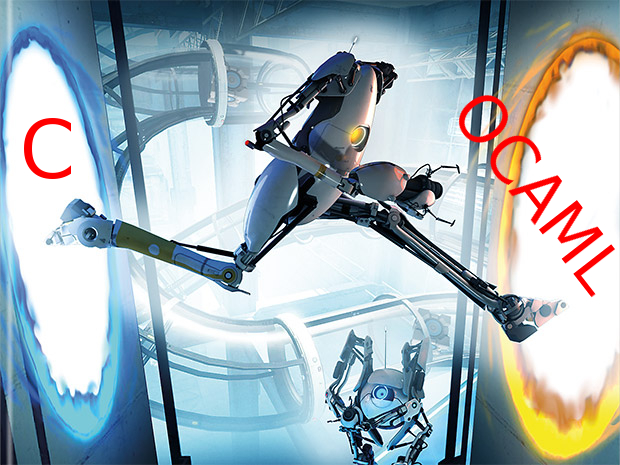
\includegraphics[scale=0.5]{COcaml.jpg}
\end{center}

Ce projet est soumis a une condition principale, très nouvelle pour nous : faire coexister le langage C avec le OCaml. Le partage entre les deux doit être relativement équitable tout au long du programme. En fait, lors du projet précédent nous avons déjà eu l'occasion de faire dialoguer les deux langages, via l'utilisation de GTK (écrit en C), notamment pour l'interface.\\

Ceci a donc été la principale raison qui nous a pousse a faire l'interface de ce projet-ci en Caml. L'interface entièrement en OCaml doit donc appeler des fonctions, comme la lecture d'un fichier, en C.\\

Tous les types OCaml sont exportés dans le monde C avec le type unique "value". On convertit ensuite les valeurs de ce type en données manipulables par le C, et on renvoie une valeur qui, elle aussi, doit être de type "value". Le code C et le code OCaml sont placés dans des fichiers séparés qui diffèrent par leur nom. En effet, a la compilation, deux fichiers .o seront générés ayant le même nom, un pour la version en Ocaml et l'autre en C. Ceci posera alors problème. On ne fait que appeler du C a partir du OCaml.\\

Comme il a été dit plus haut, c'est l'interface qui est codée en OCaml. C'est lorsque l'utilisateur veut lire une musique que le programme appelle une fonction en C. Le bouton "play" de l'interface, code en Ocaml, appelle une fonction en C dans un autre fichier qui va lire le fichier musical choisi.\\

L'un des problèmes majeurs auquel nous avons été confronte fut la compilation. En effet, puisque nous utilisons une libraire externe, FMOD donc, nous n'avons pas pu faire le lien directement via les commandes de compilations habituelles, notamment l'utilisation des .o, car OCamlc ne peut utiliser en même temps les .o et les .so (produit par FMOD) pour produire les exécutables. Il a donc fallu mettre notre code C dans sa propre librairie qui sert de lien avec l'OCaml, la compilation intégrant notre librairie de liens.\\

Actuellement, les fonctions stop, pause, volume et de chargement de fichier utilisent enfin le dialogue C - OCaml. En effet, elles utilisent chacune des fonctions de FMOD qui ne sont disponibles qu'en C.

\chapter{ La playlist}

Une liste d'écoute, aussi appelée liste de lecture ou playlist, est un ensemble de morceaux musicaux ou de fichiers audio/vidéo compilés dans un agrégateur. Ils peuvent être joués séquentiellement, dans un ordre aléatoire ou selon une logique choisie par celui qui l'a composée.

Le terme est notamment utilisé dans le monde de la radio, pour désigner la liste de morceaux en rotation sur les ondes et par les DJ pour désigner leur sélection de morceaux (faisant souvent partie d'un mix) lors d'une prestation ou d'une diffusion.
Les termes de liste de lecture et de playlist sont utilisés de façon de plus en plus fréquente pour désigner une liste de morceaux compilés sur un ordinateur personnel et destinés à être joués ou transférés sur un baladeur numérique.


\begin{center}
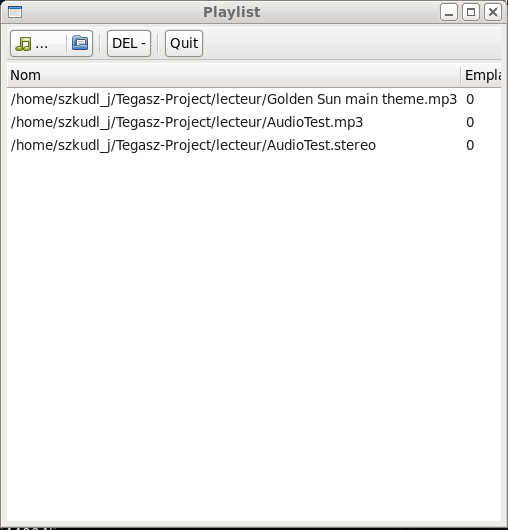
\includegraphics[scale=1]{playlist.png}
\it{interface de liste de lecture}
\end{center}

\section{utilisation}
la playlist permet à l'utilisateur de se créer une compilation de morceaux qui s'enchaineront les uns après les autres. La fenêtre est composée de trois parties principales, la liste, permettant d'afficher les morceaux ajoutés pas l'utilisateur, un bouton "add" permettant d'ajouter une élément à la liste sans influencer la lecture en cours et un bouton "delete" pour enlever des éléments et ainsi gérer facilement la liste de lecture.

\section{création de la playlist}


\chapter{la pochette}

Une pochette est l'emballage d'un album de musique. Selon le support de l'enregistrement, le terme peut se référer à une impression sur papier cartonné pour les disques vinyles (carré de 12,375 pouces pour les 33 tours), ou plus récemment à l'emballage en papier cartonné ou en matière plastique des CD.

\begin{center}

\includegraphics[scale=0.7]{cover.png}
\it{interface de liste de lecture}
\end{center}

Cette fenêtre est exclusivement composée par la pochette de l'album en cours.
Nous récupérons les données incluses dans les métas données du fichier audio. 
Si ce dernier contient le nom d'un album, nous envoyons ce dernier au code en Caml. 
Nous recherchons ensuite le nom de l'album en dans le dossier. l'image trouvée, celle ci s'affiche dans la page.

\chapter{site web}


\chapter{Conclusion}


\begin{center}
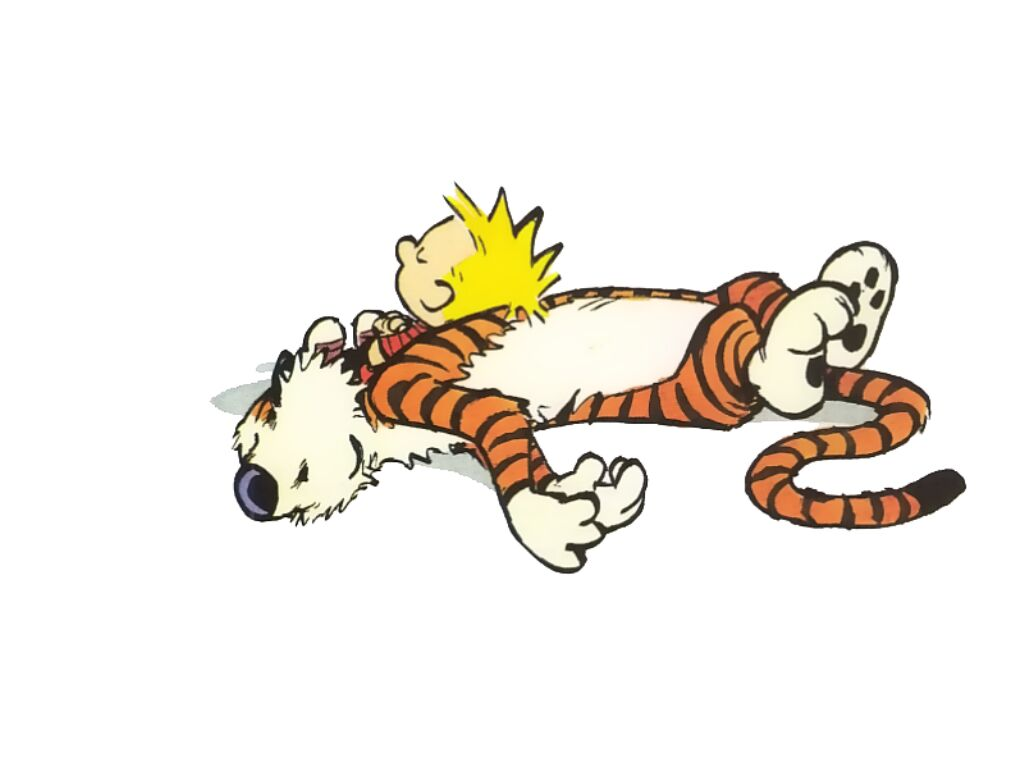
\includegraphics[scale =0.5]{conclu.jpg}
\end{center}
\end{document}
